\subsubsection{Network-Flow-Based Fair Approach}\label{NFBFA}
~

Network-Flow-Base Greedy Approach only ensures that the sum data transferring time of $k$ tasks is minimized. However, it does not achieve max-min fairness and may suffer from same problem as Greedy Approach. Here, we introduce a Network-Flow-Based Fair Approach, which can achieve max-min fairness.

\textbf{Construction}. We construct the network graph similar to Network-Flow-Based Greedy Approach. But take both data transferring time and execute time into consideration (i.e. $w_e=c^k_{i,j}+e^k_{i,j}$).  

\textbf{Solve}. To achieve max-min fairness, we need first to minimize $\max\{c^k_{i,j}+e^k_{i,j}\}$. It is quite hard to find the optimal solution. However, to certificate it is much easier.  

Let $\Delta$ denote the answer.
\begin{enumerate}
    \item \textbf{Certifier}. Given a $\Delta$, let $G(\Delta)$ be the subgraph of $G$ consisting of only edges with $w_e\leq \Delta$. Then, we compute maximal flow in $G(\Delta)$. If $f_{max}=m$, then it indicates we can assign all dependent-free tasks within bottleneck $\Delta$.
    
    \item \textbf{Search $\Delta$}. Since, we already have a certifier. The remaining work is to find $\Delta$. We can observe that $\Delta$ is monotonic. In other words, given $\Delta_{min}$, $\Delta \geq \Delta_{min}$ are feasible solutions while $\Delta < \Delta_{min} $ are not. Thus, we can use binary search to accelerate the search of $\Delta$.
    
    \item \textbf{Max-Min Fairness}. Once we find the bottleneck of some tasks, the corresponding job's finish time can be better. Thus, we can assign other tasks (denoted by $ \mathcal{T}^{'}_{k}$) in the same job more arbitrarily as long as they do not worsen bottleneck. To achieve this, for each task in $ \mathcal{T}^{'}_{k}$, we check every corresponding edge in network graph. 
    \begin{enumerate}
        \item  If $w_e> bottleneck$, we can not bring this assignment into effect or it would worsen bottleneck. Thus, we need to set $w_e^{'}=\infty$ to ensure this edge will not be chose. 
        \item  If $w_e\leq bottleneck$, we just do the opposite and set $w_e^{'}=0$. This ensures these assignments will not affect finding bottleneck of other jobs.
    \end{enumerate}
    Moreover, we bring bottleneck assignment into effect and decrease DC capacity accordingly.
    After updating the network graph, we repeat the procedure and find the bottleneck of next job. Finally this procedure finishes when we find bottleneck of each job.
    
\end{enumerate} 
    
\begin{figure}[htb]
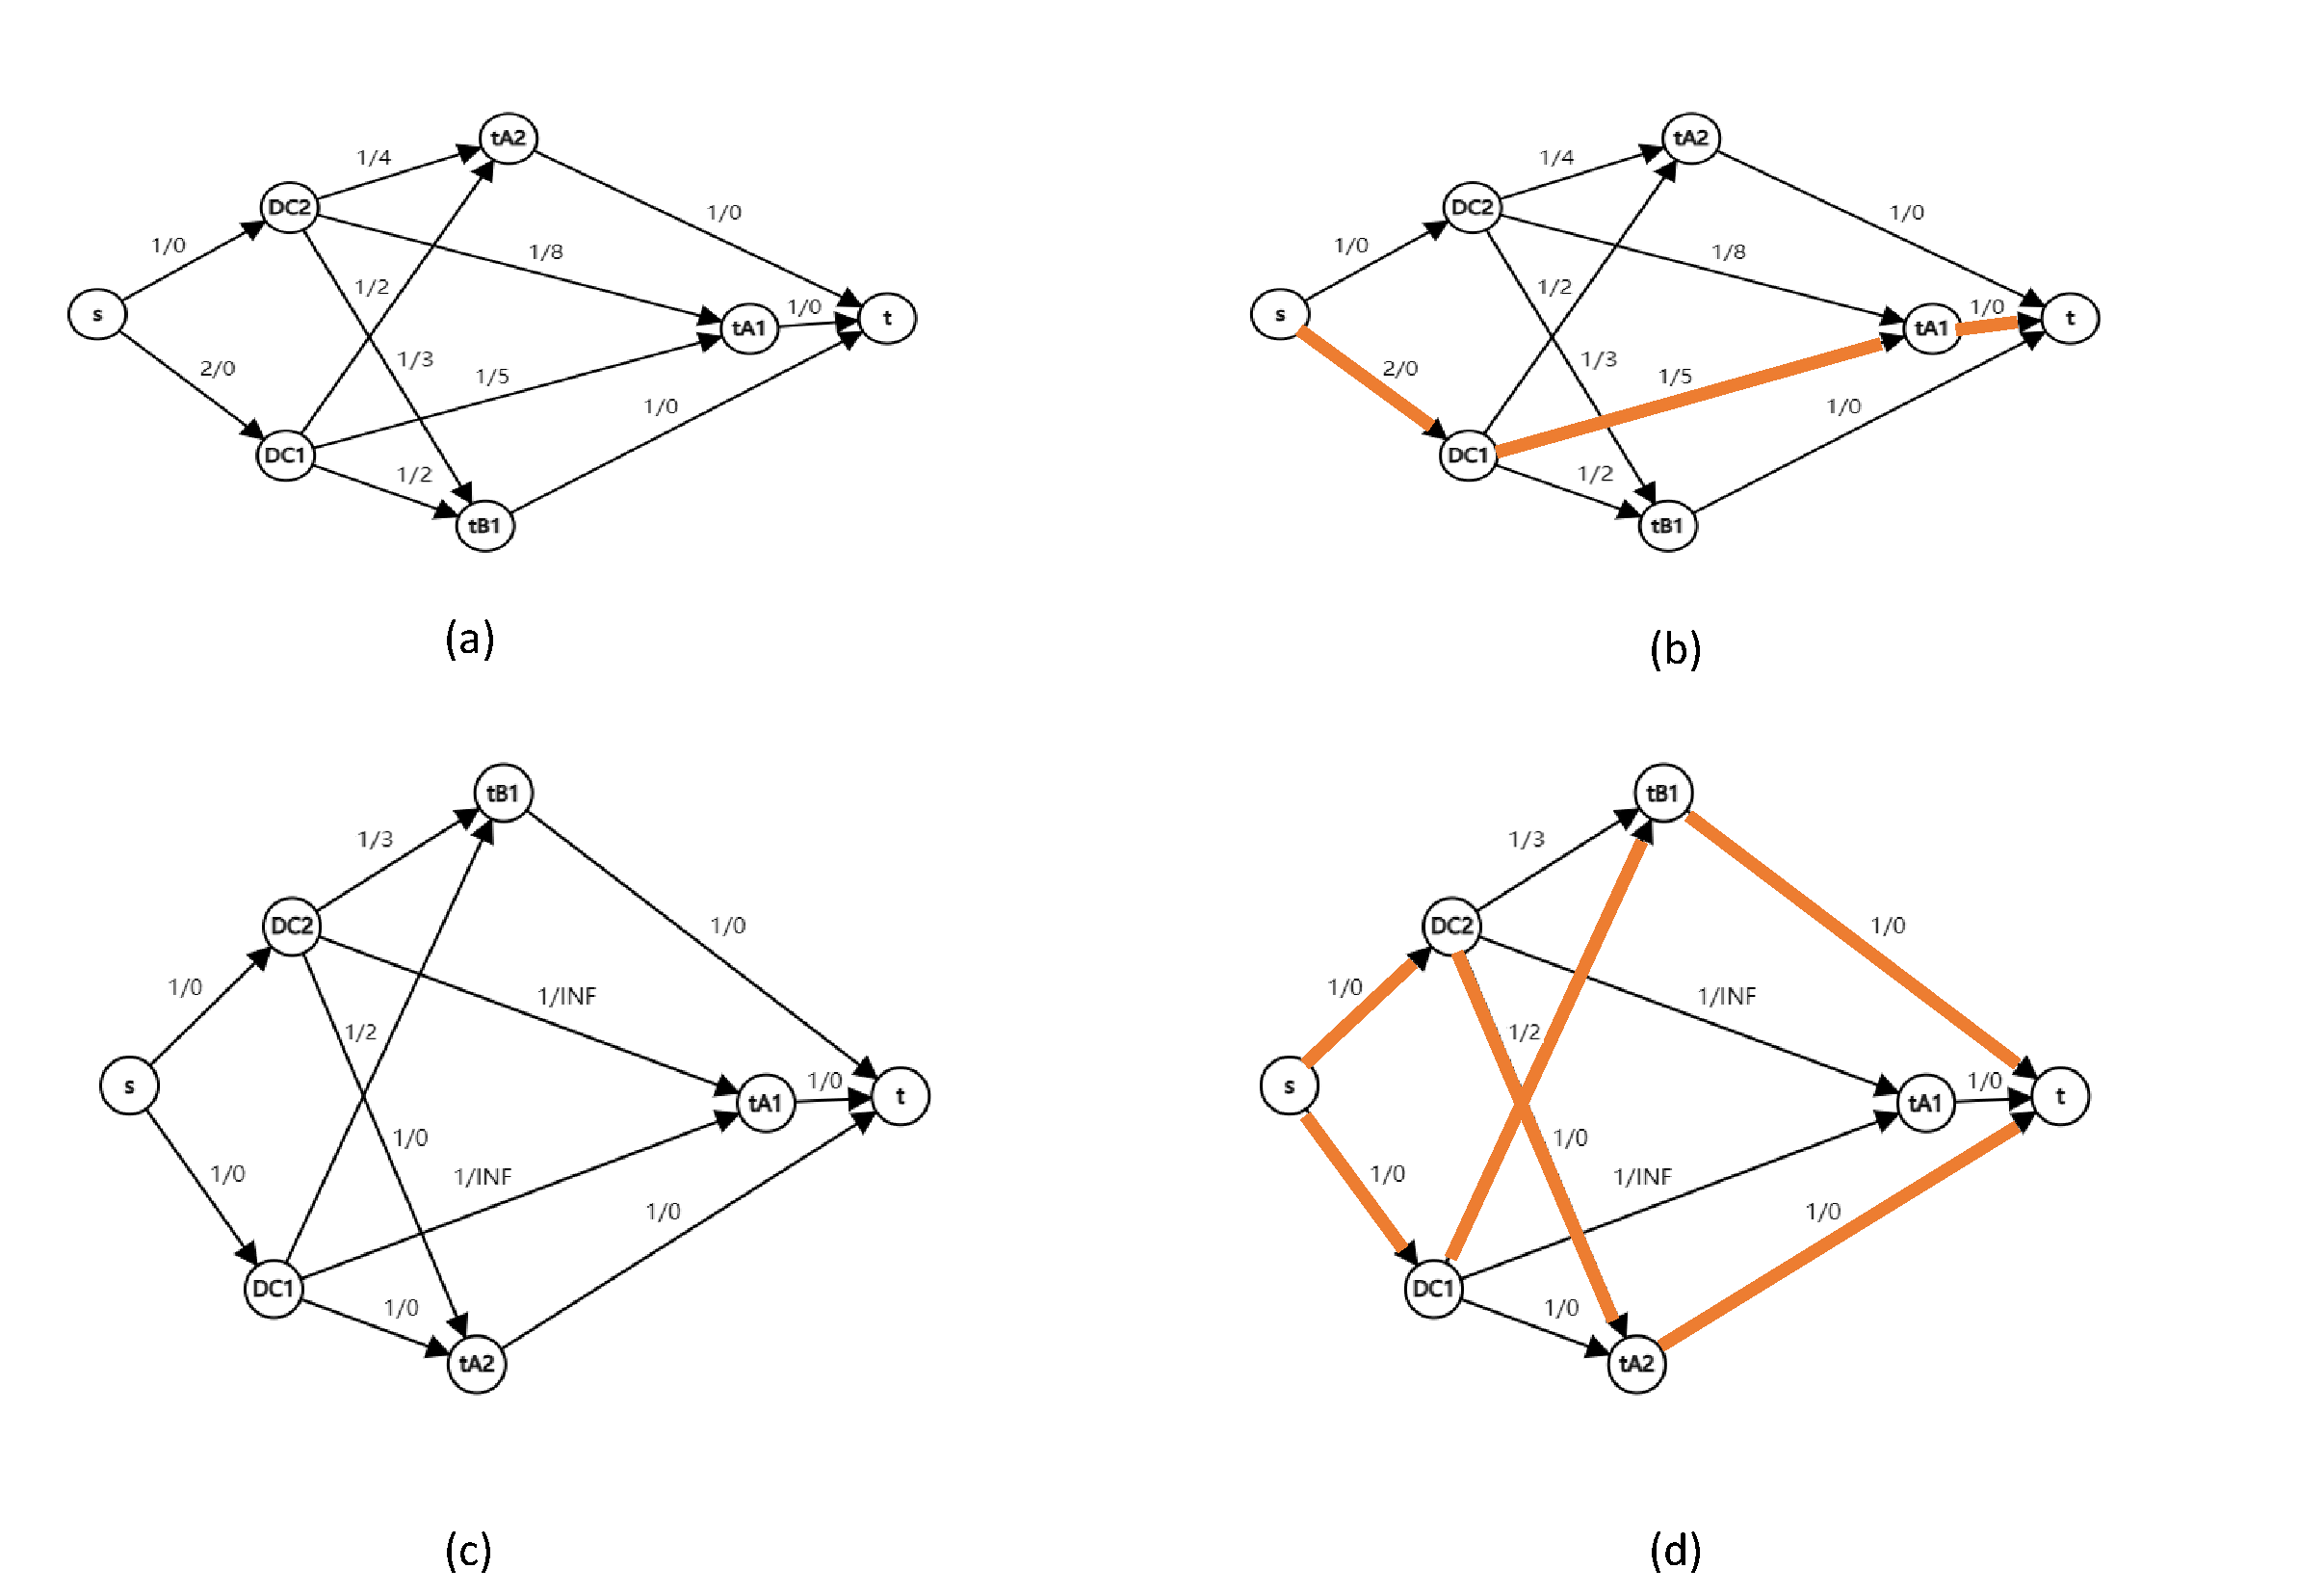
\includegraphics[width=1\textwidth]{figure/fig-fair.pdf}
\centering
\caption{Max-min fairness example.} \label{fig-fair}
\end{figure}
    
\textbf{Time Complexity}.Certifier takes $O(|J|^2m+|J|m^2)$ and binary search takes $O(\log(\max\{c_e\}) )$. Beside, we need $|\mathcal{K}|$ iterations to find bottleneck in each job respectively. Thus, the time complexity of Network-Flow-Based Fair Approach is $O((|J|^2m+|J|m^2)\log (\max \{c_e\}) |\mathcal{K}|)$.

\textbf{Example}. To illustrate better how Network-Flow-Based Fair Approach achieve max-min fairness, we introduce a new example Fig. \ref{fig-fair}. Suppose after construct we have network graph (a). We apply Network-Flow-Based Fair Approach on this and (b) shows the result of first iteration. After first iteration, we find assigning tA1 to DC1 is the bottleneck with $w_e=5$. Thus, we assign tA1 to DC1 and update the network graph accordingly. (c) shows the new network graph, where edges of job A are either $0$ or $\infty$. We repeat the procedure again and this time we find assigning tB1 to DC1 is the bottleneck with $w_e=2$. As there are only 2 jobs and we find 2 bottlenecks, the algorithm terminates with max-min fairness solution (tA1,tA2,tB1)$=(5,4,2)$.
Note that Greedy Base Approach can never give this solution as $(5,2,3)$ minimize the sum completion time.
    
